% https://tex.stackexchange.com/a/563998/240347
\begin{figure}
    \centering
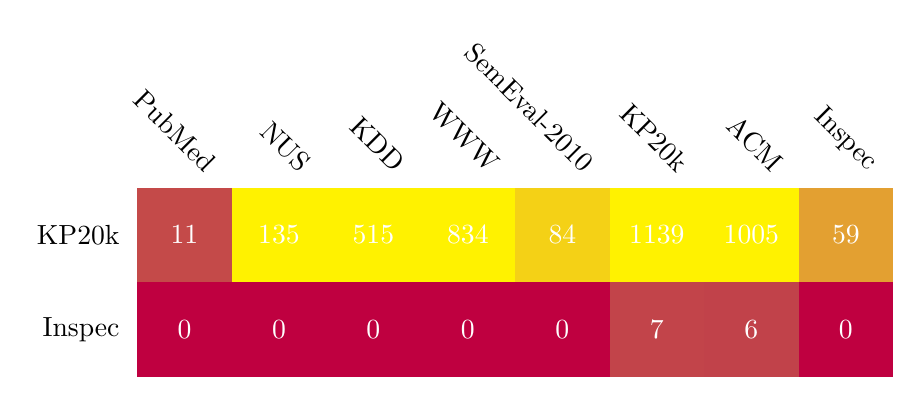
\begin{tikzpicture}[scale=1.2]
  %\node at (5,0) {Heatmap of Nodes};
  \foreach \x [count=\n] in {
        PubMed,NUS,KDD,WWW,SemEval-2010,KP20k,ACM,Inspec
  } {
       \node[rotate=-45,xshift=0.6cm,anchor=east] at (\n,0) {\x};
  }
  \foreach \y [count=\n] in {
        KP20k, Inspec
  } {
       \node[xshift=0.5cm,anchor=east] at (0,-\n) {\y};
  }
  \foreach \y [count=\n] in {
        {11, 135, 515, 834, 84, 1139, 1005, 59},
        { 0,   0,   0,   0,  0,    7,    6,  0},
    } {
      \foreach \x [count=\m] in \y {
        \node[fill=yellow!\x!purple, minimum size=12mm, text=white] at (\m,-\n) {\x};
      }
    }
\end{tikzpicture}
    \caption{Nombre de document commun entre les ensembles d'entraînement de KP20k et Inspec et les ensembles de test.}
    \label{fig:heatmap_train_test}
\end{figure}



% https://texblog.org/2013/06/13/latex-heatmap-using-tabular/
\iffalse
\newcommand*{\MinNumber}{0}%
\newcommand*{\MaxNumber}{1}%
 
\newcommand{\ApplyGradient}[1]{%
        \pgfmathsetmacro{\PercentColor}{100.0*(#1-\MinNumber)/(\MaxNumber-\MinNumber)}
        \hspace{-0.33em}\colorbox{red!\PercentColor!black}{}
}
 
\newcolumntype{R}{>{\collectcell\ApplyGradient}c<{\endcollectcell}}
\renewcommand{\arraystretch}{0}
\setlength{\fboxsep}{3mm} % box size
\setlength{\tabcolsep}{0pt}

\begin{table}[ht]
    \begin{center}
    \begin{tabular}{l*{8}{R}}
        \toprule
        %{} &  {PubMed} &  {KDD} &  {WWW} &  {SemEval-2010} &  {KP20k} &  {NTCIR1+2} &  {ACM} &  {Inspec} \\
        \midrule
        {KP20k}  & 11 & 515 & 834 & 84 & 1139 & 72 & 1005 & 59 \\
        {Inspec} &  0 &   0 &   0 &  0 &    7 &  0 &    6 &  0 \\
        \bottomrule
    \end{tabular}
    \end{center}
\end{table}
\fi

% https://tex.stackexchange.com/a/83865/240347
\iffalse
\pgfplotstableset{
    /color cells/min/.initial=0,
    /color cells/max/.initial=1000,
    /color cells/textcolor/.initial=,
    %
    % Usage: 'color cells={min=<value which is mapped to lowest color>, 
    %   max = <value which is mapped to largest>}
    color cells/.code={%
        \pgfqkeys{/color cells}{#1}%
        \pgfkeysalso{%
            postproc cell content/.code={%
                %
                \begingroup
                %
                % acquire the value before any number printer changed
                % it:
                \pgfkeysgetvalue{/pgfplots/table/@preprocessed cell content}\value
                \ifx\value\empty
                    \endgroup
                \else
                \pgfmathfloatparsenumber{\value}%
                \pgfmathfloattofixed{\pgfmathresult}%
                \let\value=\pgfmathresult
                %
                % map that value:
                \pgfplotscolormapaccess
                    [\pgfkeysvalueof{/color cells/min}:\pgfkeysvalueof{/color cells/max}]
                    {\value}
                    {\pgfkeysvalueof{/pgfplots/colormap name}}%
                % now, \pgfmathresult contains {<R>,<G>,<B>}
                % 
                % acquire the value AFTER any preprocessor or
                % typesetter (like number printer) worked on it:
                \pgfkeysgetvalue{/pgfplots/table/@cell content}\typesetvalue
                \pgfkeysgetvalue{/color cells/textcolor}\textcolorvalue
                %
                % tex-expansion control
                % see https://tex.stackexchange.com/questions/12668/where-do-i-start-latex-programming/27589#27589
                \toks0=\expandafter{\typesetvalue}%
                \xdef\temp{%
                    \noexpand\pgfkeysalso{%
                        @cell content={%
                            \noexpand\cellcolor[rgb]{\pgfmathresult}%
                            \noexpand\definecolor{mapped color}{rgb}{\pgfmathresult}%
                            \ifx\textcolorvalue\empty
                            \else
                                \noexpand\color{\textcolorvalue}%
                            \fi
                            \the\toks0 %
                        }%
                    }%
                }%
                \endgroup
                \temp
                \fi
            }%
        }%
    }
}



\begin{table}\caption{Correlation or something}
    \centering
    \pgfplotstabletypeset[
    color cells={min=-300,max=800},
    col sep=comma,
    %/pgfplots/colormap={whiteblue}{rgb255(0cm)=(255,255,255); rgb255(1cm)=(0,0,188)},
]{
        PubMed,KDD,WWW,SemEval-2010,KP20k,NTCIR1+2,ACM,Inspec
          11, 515, 834, 84, 1139, 72, 1005, 59
          0,   0,   0,  0,    7,  0,    6,  0
    }
\end{table}
\fi